% Compile with XeLaTeX, TeXLive 2013 or more recent
\documentclass{beamer}

% Base packages
\usepackage{fontspec}
\usepackage{xunicode}
\usepackage{xltxtra}

\usepackage{amsfonts}
\usepackage{amsmath}
\usepackage{longtable}
\usepackage{csquotes}
\usepackage{standalone}

% Setup fonts
\newfontfamily\russianfont{CMU Serif}
\setromanfont{CMU Serif}
\setsansfont{CMU Sans Serif}
\setmonofont{CMU Typewriter Text}

% Setup Russian hyphenation. NOTE: this declaration *must* come after fontspec's font declarations,
% or a mysterious (but harmless in other respects) error "Improper `at' size (0.0pt), replaced by 10pt." would appear.
\usepackage{polyglossia}
\defaultfontfeatures{Scale=MatchLowercase, Mapping=tex-text}

\setdefaultlanguage[spelling=modern]{russian} % for polyglossia
\setotherlanguage{english} % for polyglossia

% Vector drawings 
\usepackage{tikz}
\usetikzlibrary{shapes, calc, arrows, fit, positioning, decorations, patterns, decorations.pathreplacing, chains, snakes}

% Be able to insert hyperlinks
\usepackage{hyperref}
\hypersetup{colorlinks=true, linkcolor=black, filecolor=black, citecolor=black, urlcolor=blue , pdfauthor=Grigory Rechistov <grigory.rechistov@phystech.edu>, pdftitle=Моделирование OpenRISC 1000 на Wind River Simics}
% \usepackage{url}

% Misc optional packages
\usepackage{underscore}
\usepackage{amsthm}

% A new command to mark not done places
\newcommand{\todo}[1][Напиши меня]{{\color{red}TODO\ #1}}


\title{Краткое введение в OpenRISC 1000}
% \subtitle{Курс «Программное моделирование вычислительных систем»}
\subject{Лекция}
\author[Григорий Речистов]{Григорий Речистов \\ \small{\href{mailto:grigory.rechistov@intel.com}{grigory.rechistov@intel.com}}}
\date{\today}
\pgfdeclareimage[height=0.5cm]{intel-logo}{../images/intel.png}
\logo{\pgfuseimage{intel-logo}}


\typeout{Copyright 2014 Grigory Rechistov}

\usetheme{Berlin}
\setbeamertemplate{navigation symbols}{}%remove navigation symbols

\begin{document}

\begin{frame}
\titlepage
\end{frame}

\begin{frame}
\tableofcontents
\end{frame} 


\section{Обзор}

\begin{frame}{Что такое OpenRISC}

\todo

\end{frame}

\begin{frame}{Почему OpenRISC для симуляции}

\end{frame}

\begin{frame}{ISA}

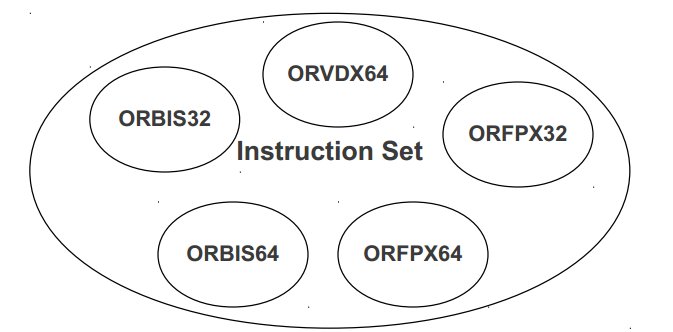
\includegraphics[width=0.8\textwidth]{./or1k-isa}

% \begin{tikzpicture}[>=latex]

% \end{tikzpicture}
\end{frame}



\section{Литература}

\begin{frame}[allowframebreaks]{Литература}
\begin{thebibliography}{99}
    \bibitem{simbook} Основы программного моделирования ЭВМ. Учебное пособие / Г. Речистов, А. Иванов, П. Шишпор, Н. Щелкунов, Д. Гаврилов, В. Пентковский. — Издательство МФТИ, дек. 2012. — ISBN 978-5-7417-0469-1

\end{thebibliography}
\end{frame}


\section{Конец}
% The final "thank you" frame 
\begin{frame}

{\huge{Спасибо за внимание!}\par}

\vfill

Слайды и материалы курса доступны по адресу \url{http://bit.ly/1y1lZF1} % http://atakua.doesntexist.org/wordpress/tag/or1k/

\vfill

\tiny{\textit{Замечание}: все торговые марки и логотипы, использованные в данном материале, являются собственностью их владельцев. Представленная точка зрения отражает личное мнение автора.
%Материалы доступны по лицензии Creative Commons Attribution-ShareAlike (Атрибуция — С сохранением условий) 4.0 весь мир (в т.ч. Россия и др.). Чтобы ознакомиться с экземпляром этой лицензии, посетите \url{http://creativecommons.org/licenses/by-sa/4.0/}
}

\end{frame}

% \section{Резерв}

\end{document}
